% answers.tex —— 2010 年·普通高等学校招生考试·安徽卷·文科 · 参考答案与详细解析片段
% 由 tools/generate_projects.py 依来源总账自 2010/2010_数学真题_安徽文_试题.md + 2010/2010_数学真题_安徽文_解析正文.md + 2010/2010_数学真题_安徽文_答案要点.md 生成，勿手改（改源 MD 后重跑）


\begin{gktip}
固定候选 PDF 仅含题面，无答案、解析和评分标准，原页亦未标分值；以下为非官方编者独立推导，官方答案字段为空。分数、根号、上下标与六幅图均以 600 dpi 原页复核。
\end{gktip}

\begin{answer}
\gksolhead{1}{}

\textbf{题目}：

若 $A=\{x\mid x+1>0\}$，$B=\{x\mid x-3<0\}$，则 $A\cap B=$（　）

（A）$(-1,+\infty)$

（B）$(-\infty,3)$

（C）$(-1,3)$

（D）$(1,3)$

\Needspace{4\baselineskip}
\textbf{解析}

分别解两个一次不等式，再取交集。

$A=(-1,+\infty)$，$B=(-\infty,3)$，故 $A\cap B=(-1,3)$，选 C。

\gkanswer{答案：C。}

\end{answer}
\begin{answer}
\gksolhead{2}{}

\textbf{题目}：

已知 $\mathrm i^2=-1$，则 $\mathrm i(1-\sqrt3\mathrm i)=$（　）

（A）$\sqrt3-\mathrm i$

（B）$\sqrt3+\mathrm i$

（C）$-\sqrt3-\mathrm i$

（D）$-\sqrt3+\mathrm i$

\Needspace{4\baselineskip}
\textbf{解析}

\Needspace{5\baselineskip}
利用 $\mathrm i^2=-1$ 展开。

\nopagebreak[4]
\[\mathrm i(1-\sqrt3\mathrm i)=\mathrm i-\sqrt3\mathrm i^2=\sqrt3+\mathrm i.\]

选 B。

\gkanswer{答案：B。}

\end{answer}
\begin{answer}
\gksolhead{3}{}

\textbf{题目}：

设向量 $\boldsymbol a=(1,0)$，$\boldsymbol b=\left(\dfrac12,\dfrac12\right)$，则下列结论中正确的是（　）

（A）$|\boldsymbol a|=|\boldsymbol b|$

（B）$\boldsymbol a\cdot\boldsymbol b=\dfrac{\sqrt2}2$

（C）$\boldsymbol a\parallel\boldsymbol b$

（D）$\boldsymbol a-\boldsymbol b$ 与 $\boldsymbol b$ 垂直

\Needspace{4\baselineskip}
\textbf{解析}

逐个计算模、数量积与平行、垂直关系。

\Needspace{5\baselineskip}
$|\boldsymbol a|=1$，$|\boldsymbol b|=\sqrt{\dfrac14+\dfrac14}=\dfrac{\sqrt2}2$，故 A 错；$\boldsymbol a\cdot\boldsymbol b=\dfrac12$，故 B 错；两向量的对应分量不成比例，故 C 错；而

\nopagebreak[4]
\[(\boldsymbol a-\boldsymbol b)\cdot\boldsymbol b
=\left(\frac12,-\frac12\right)\cdot\left(\frac12,\frac12\right)=0,\]

故 D 正确。选 D。

\gkanswer{答案：D。}

\end{answer}
\begin{answer}
\gksolhead{4}{}

\textbf{题目}：

过点 $(1,0)$ 且与直线 $x-2y-2=0$ 平行的直线方程是（　）

（A）$x-2y-1=0$

（B）$x-2y+1=0$

（C）$2x+y-2=0$

（D）$x+2y-1=0$

\Needspace{4\baselineskip}
\textbf{解析}

平行直线的一次项系数相同，只需确定常数项。

设所求直线为 $x-2y+C=0$。代入点 $(1,0)$ 得 $1-0+C=0$，即 $C=-1$。故直线为 $x-2y-1=0$。选 A。

\gkanswer{答案：A。}

\end{answer}
\begin{answer}
\gksolhead{5}{}

\textbf{题目}：

设数列 $\{a_n\}$ 的前 $n$ 项和 $S_n=n^2$，则 $a_8$ 的值为（　）

（A）$15$

（B）$16$

（C）$49$

（D）$64$

\Needspace{4\baselineskip}
\textbf{解析}

\Needspace{5\baselineskip}
用 $a_n=S_n-S_{n-1}$（$n\geqslant2$）计算。

\nopagebreak[4]
\[a_8=S_8-S_7=64-49=15.\]

选 A。

\gkanswer{答案：A。}

\end{answer}
\begin{answer}
\gksolhead{6}{}

\textbf{题目}：

设 $abc>0$，二次函数 $f(x)=ax^2+bx+c$ 的图象可能是（　）
\nopagebreak[4]
\begin{center}% 2010 年安徽卷文科第 6 题：四个二次函数图象选项（A）—（D）。
% 来源 PDF：普通高考/2010/2010安徽文.pdf，SHA-256 1bd928e09356787e648fa9efb9b4c1525f26334f65b08ba82fc736ebb110a4cb。
% 原页：第 1 页（A3 三栏）第 1 栏中部，书页码 571。
% 重绘依据：四幅均只示意开口方向、y 轴截距符号与对称轴位置，不标刻度：
%   (A) 开口向下、截距为负、对称轴在 y 轴左侧；(B) 开口向下、截距为正、对称轴在右侧；
%   (C) 开口向上、截距为负、对称轴在左侧；(D) 开口向上、截距为负、对称轴在右侧。
\begin{tikzpicture}[semithick, scale=1.15, every node/.style={inner sep=1.2pt, font=\small}]
  % (A)
  \begin{scope}[shift={(0,0)}]
    \draw[-stealth] (-1.75,0) -- (0.75,0) node[right] {$x$};
    \draw[-stealth] (0,-0.95) -- (0,0.65) node[above] {$y$};
    \draw[thick,domain=-1.55:0.30,samples=80] plot (\x,{-0.8*(\x+0.7)^2+0.4});
    \node[below] at (-0.35,-1.35) {（A）};
  \end{scope}
  % (B)
  \begin{scope}[shift={(3.3,0)}]
    \draw[-stealth] (-0.55,0) -- (1.95,0) node[right] {$x$};
    \draw[-stealth] (0,-0.65) -- (0,0.95) node[above] {$y$};
    \draw[thick,domain=-0.45:1.85,samples=80] plot (\x,{-0.8*(\x-0.7)^2+0.7});
    \node[below] at (0.7,-1.35) {（B）};
  \end{scope}
  % (C)
  \begin{scope}[shift={(0,-3.1)}]
    \draw[-stealth] (-1.65,0) -- (0.65,0) node[right] {$x$};
    \draw[-stealth] (0,-0.75) -- (0,0.65) node[above] {$y$};
    \draw[thick,domain=-1.50:0.40,samples=80] plot (\x,{0.8*(\x+0.6)^2-0.5});
    \node[below] at (-0.45,-1.35) {（C）};
  \end{scope}
  % (D)
  \begin{scope}[shift={(3.3,-3.1)}]
    \draw[-stealth] (-0.40,0) -- (1.95,0) node[right] {$x$};
    \draw[-stealth] (0,-0.70) -- (0,0.75) node[above] {$y$};
    \draw[thick,domain=-0.30:1.80,samples=80] plot (\x,{0.8*(\x-0.75)^2-0.55});
    \node[below] at (0.75,-1.35) {（D）};
  \end{scope}
\end{tikzpicture}
\end{center}
\nopagebreak[4]
\Needspace{4\baselineskip}
\textbf{解析}

由开口方向定 $a$ 的符号，由 $y$ 轴截距定 $c$ 的符号，再由对称轴位置定 $b$ 的符号。

（A）开口向下，$a<0$；$y$ 轴截距为负，$c<0$；对称轴在 $y$ 轴左侧，即 $-\dfrac b{2a}<0$，得 $b<0$。于是 $abc<0$，不合。

（B）$a<0$，$c>0$；对称轴在 $y$ 轴右侧，得 $b>0$。于是 $abc<0$，不合。

（C）$a>0$，$c<0$；对称轴在 $y$ 轴左侧，得 $b>0$。于是 $abc<0$，不合。

（D）$a>0$，$c<0$；对称轴在 $y$ 轴右侧，得 $b<0$。于是 $abc>0$，符合。

选 D。

\gkanswer{答案：D。}

\end{answer}
\begin{answer}
\gksolhead{7}{}

\textbf{题目}：

设 $a=\left(\dfrac35\right)^{\frac25}$，$b=\left(\dfrac25\right)^{\frac35}$，$c=\left(\dfrac25\right)^{\frac25}$，则 $a$，$b$，$c$ 的大小关系是（　）

（A）$a>c>b$

（B）$a>b>c$

（C）$c>a>b$

（D）$b>c>a$

\Needspace{4\baselineskip}
\textbf{解析}

把三个幂按底数、指数分别比较。

$a$ 与 $c$ 的指数同为 $\dfrac25>0$，而底数 $\dfrac35>\dfrac25$，故 $a>c$；$b$ 与 $c$ 的底数同为 $\dfrac25\in(0,1)$，而指数 $\dfrac35>\dfrac25$，故 $b<c$。因此 $a>c>b$。选 A。

\gkanswer{答案：A。}

\end{answer}
\begin{answer}
\gksolhead{8}{}

\textbf{题目}：

\Needspace{5\baselineskip}
设 $x$，$y$ 满足约束条件
\nopagebreak[4]
\[\begin{cases}2x+y-6\geqslant0,\\ x+2y-6\leqslant0,\\ y\geqslant0,\end{cases}\]
则目标函数 $z=x+y$ 的最大值是（　）

（A）$3$

（B）$4$

（C）$6$

（D）$8$

\Needspace{4\baselineskip}
\textbf{解析}

先画出可行域，再比较各顶点处的目标函数值。

三条边界直线两两相交，可行域的三个顶点为 $(3,0)$，$(6,0)$，$(2,2)$。目标函数 $z=x+y$ 在这些点的值依次为 $3$，$6$，$4$，故最大值为 $6$。选 C。

\gkanswer{答案：C。}

\end{answer}
\begin{answer}
\gksolhead{9}{}

\textbf{题目}：

一个几何体的三视图如图，该几何体的表面积为（　）
\nopagebreak[4]
\begin{center}% 2010 年安徽卷文科第 9 题：正视图、侧视图与俯视图。
% 来源 PDF：普通高考/2010/2010安徽文.pdf，SHA-256 1bd928e09356787e648fa9efb9b4c1525f26334f65b08ba82fc736ebb110a4cb。
% 原页：第 1 页（A3 三栏）第 2 栏上部，书页码 571。
% 重绘依据：正视图总宽 8（上部宽 6、两侧各 1），上部高 8、底座高 2；
%   侧视图总宽 10（6、2、2），上部宽 2；俯视图外框 8×10，内框 6×2 位于距上边 6 处。
\begin{tikzpicture}[semithick, scale=0.72, every node/.style={inner sep=1.2pt, font=\small}]
  % 正视图
  \draw (0,0) rectangle (8,2);
  \draw (1,2) rectangle (7,10);
  \draw[<->] (0,10.5) -- (1,10.5) node[midway,above] {$1$};
  \draw[<->] (1,10.5) -- (7,10.5) node[midway,above] {$6$};
  \draw[<->] (7,10.5) -- (8,10.5) node[midway,above] {$1$};
  \draw[<->] (-0.45,2) -- (-0.45,10) node[midway,left] {$8$};
  \draw[<->] (-0.45,0) -- (-0.45,2) node[midway,left] {$2$};
  \node[below] at (4,-0.55) {正（主）视图};
  % 侧视图
  \draw (10,0) rectangle (20,2);
  \draw (16,2) rectangle (18,10);
  \draw[<->] (10,10.5) -- (16,10.5) node[midway,above] {$6$};
  \draw[<->] (16,10.5) -- (18,10.5) node[midway,above] {$2$};
  \draw[<->] (18,10.5) -- (20,10.5) node[midway,above] {$2$};
  \node[below] at (15,-0.55) {侧（左）视图};
  % 俯视图
  \draw (0,-14) rectangle (8,-4);
  \draw (1,-12) rectangle (7,-10);
  \draw[<->] (-0.45,-4) -- (-0.45,-10) node[midway,left] {$6$};
  \draw[<->] (-0.45,-10) -- (-0.45,-12) node[midway,left] {$2$};
  \draw[<->] (-0.45,-12) -- (-0.45,-14) node[midway,left] {$2$};
  \node[below] at (4,-14.55) {俯视图};
\end{tikzpicture}
\end{center}
\nopagebreak[4]
\begin{gkopts}(4)
\task （A）$372$
\task （B）$360$
\task （C）$292$
\task （D）$280$
\end{gkopts}

\Needspace{4\baselineskip}
\textbf{解析}

先由三视图还原组合体，再计算表面积。

\Needspace{5\baselineskip}
下方是 $8\times10\times2$ 的长方体，上方是 $6\times2\times8$ 的长方体，两者接触面为 $6\times2$。故表面积

\nopagebreak[4]
\[S=2(80+16+20)+2(12+48+16)-2\times12=232+152-24=360.\]

选 B。

\gkanswer{答案：B。}

\end{answer}
\begin{answer}
\gksolhead{10}{}

\textbf{题目}：

甲从正方形四个顶点中任意选择两个顶点连成直线，乙也从该正方形四个顶点中任意选择两个顶点连成直线，则所得的两条直线相互垂直的概率是（　）

\begin{gkopts}(4)
\task （A）$\dfrac3{18}$
\task （B）$\dfrac3{18}$
\task （C）$\dfrac5{18}$
\task （D）$\dfrac6{18}$
\end{gkopts}

\Needspace{4\baselineskip}
\textbf{解析}

先数总结果数，再数两条直线互相垂直的有序结果数。

每人有 $\mathrm C_4^2=6$ 种选法，故共有 $36$ 个等可能的有序结果。两条直线为正方形的边或对角线：相邻两边垂直，共 $4\times2=8$ 个有序结果；两条对角线互相垂直，共 $2$ 个有序结果。故所求概率为 $\dfrac{8+2}{36}=\dfrac5{18}$。选 C。

原页选项（A）与（B）均印作 $\dfrac3{18}$，此处照录，不影响唯一正确选项。

\gkanswer{答案：C。}

\end{answer}
\begin{answer}
\gksolhead{11}{}

\textbf{题目}：

命题“存在 $x\in\mathbf R$，使得 $x^2+2x+5=0$”的否定是$\underline{\qquad}$。

\Needspace{4\baselineskip}
\textbf{解析}

特称命题的否定是全称命题：把“存在”改为“任意”，并否定结论。

故否定为：对任意 $x\in\mathbf R$，都有 $x^2+2x+5\neq0$。

\gkanswer{答案：对任意 $x\in\mathbf R$，都有 $x^2+2x+5\neq0$。}

\end{answer}
\begin{answer}
\gksolhead{12}{}

\textbf{题目}：

抛物线 $y^2=4x$ 的焦点坐标是$\underline{\qquad}$。

\Needspace{4\baselineskip}
\textbf{解析}

把方程与标准形式 $y^2=2px$ 对照。

由 $2p=4$ 得 $p=2$，焦点坐标为 $\left(\dfrac p2,0\right)=(1,0)$。

\gkanswer{答案：$(1,0)$。}

\end{answer}
\begin{answer}
\gksolhead{13}{}

\textbf{题目}：

如图所示，程序框图（算法流程图）的输出值 $x=$ $\underline{\qquad}$。
\nopagebreak[4]
\begin{center}% 2010 年安徽卷文科第 13 题：算法流程图。
% 来源 PDF：普通高考/2010/2010安徽文.pdf，SHA-256 1bd928e09356787e648fa9efb9b4c1525f26334f65b08ba82fc736ebb110a4cb。
% 原页：第 1 页（A3 三栏）第 2 栏中部，书页码 571。
% 重绘依据：开始 → x=1 → 判断「x 是奇数?」；是（右）→ x=x+1 → 回到判断前；
%   否（下）→ x=x+2 → 判断「x>8?」；否（右）→ 回到「x 是奇数?」前；是（下）→ 输出 x → 结束。
\begin{tikzpicture}[semithick, >=Stealth,
  every node/.style={inner sep=1.5pt, font=\small}]
  \node (start) [draw, rounded corners=4pt, minimum width=1.9cm, minimum height=0.55cm] at (0,0) {开始};
  \node (x1) [draw, minimum width=1.9cm, minimum height=0.55cm] at (0,-1.35) {$x=1$};
  \node (c1) [draw, diamond, aspect=2.1, minimum width=3.1cm,
    minimum height=1.15cm] at (0,-3.15) {$x$ 是奇数?};
  \node (p1) [draw, minimum width=2.5cm, minimum height=0.55cm] at (3.7,-3.15) {$x=x+1$};
  \node (p2) [draw, minimum width=2.5cm, minimum height=0.55cm] at (0,-4.85) {$x=x+2$};
  \node (c2) [draw, diamond, aspect=2.1, minimum width=3.1cm,
    minimum height=1.15cm] at (0,-6.65) {$x>8?$};
  \node (out) [draw, trapezium, trapezium left angle=72, trapezium right angle=108,
    minimum width=2.4cm, minimum height=0.55cm] at (0,-8.25) {输出 $x$};
  \node (end) [draw, rounded corners=4pt, minimum width=1.9cm, minimum height=0.55cm] at (0,-9.45) {结束};

  \draw[->] (start) -- (x1);
  \draw[->] (x1) -- (c1);
  \draw[->] (c1.east) -- node[above] {是} (p1.west);
  \draw[->] (c1.south) -- node[right] {否} (p2.north);
  \draw[->] (p2) -- (c2);
  \draw[->] (c2.south) -- node[right] {是} (out.north);
  \draw[->] (out) -- (end);
  % x=x+1 的回流
  \draw (p1.north) -- (3.7,-2.0) -- (0,-2.0);
  % x>8? 为否时的回流
  \draw (c2.east) -- node[above] {否} (5.2,-6.65) -- (5.2,-2.0) -- (0,-2.0);
  \draw[->] (0,-2.0) -- (c1.north);
\end{tikzpicture}
\end{center}
\nopagebreak[4]
\Needspace{4\baselineskip}
\textbf{解析}

按框图顺序逐步执行，注意判断为“是”与“否”时的不同去向。

初始 $x=1$。$1$ 为奇数，执行 $x=x+1$ 得 $2$；$2>8$ 不成立，继续。$2$ 为偶数，执行 $x=x+2$ 得 $4$；$4>8$ 不成立。$4$ 为偶数，得 $6$；$6>8$ 不成立。$6$ 为偶数，得 $8$；$8>8$ 不成立。$8$ 为偶数，得 $10$；此时 $10>8$ 成立，输出 $x=10$。

\gkanswer{答案：$10$。}

\end{answer}
\begin{answer}
\gksolhead{14}{}

\textbf{题目}：

某地有居民 $100000$ 户，其中普通家庭 $99000$ 户，高收入家庭 $1000$ 户。从普通家庭中以简单随机抽样方式抽取 $990$ 户，从高收入家庭中以简单随机抽样方式抽取 $100$ 户进行调查，发现共有 $120$ 户家庭拥有 $3$ 套或 $3$ 套以上住房，其中普通家庭 $50$ 户，高收入家庭 $70$ 户。依据这些数据并结合所掌握的统计知识，你认为该地拥有 $3$ 套或 $3$ 套以上住房的家庭所占比例的合理估计是$\underline{\qquad}$。

\Needspace{4\baselineskip}
\textbf{解析}

用样本中拥有 $3$ 套或 $3$ 套以上住房的户数占样本总户数的比例作估计。

\Needspace{5\baselineskip}
样本共 $990+100=1090$ 户，其中 $120$ 户拥有 $3$ 套或 $3$ 套以上住房，故合理估计为

\nopagebreak[4]
\[\frac{120}{1090}=\frac{12}{109}\approx0.110,\]

即约 $11\%$。

\gkanswer{答案：$11\%$（即 $\dfrac{12}{109}$）。}

\end{answer}
\begin{answer}
\gksolhead{15}{}

\textbf{题目}：

若 $a>0$，$b>0$，$a+b=2$，则下列不等式对一切满足条件的 $a$，$b$ 恒成立的是$\underline{\qquad}$。（写出所有正确命题的编号）

① $ab\leqslant1$；

② $\sqrt a+\sqrt b\leqslant\sqrt2$；

③ $a^2+b^2\geqslant2$；

④ $a^3+b^3\geqslant3$；

⑤ $\dfrac1a+\dfrac1b\geqslant2$。

\Needspace{4\baselineskip}
\textbf{解析}

利用 $a+b=2$ 与基本不等式逐项判断。

① 由 $ab\leqslant\left(\dfrac{a+b}2\right)^2=1$，正确。

② $(\sqrt a+\sqrt b)^2=2+2\sqrt{ab}>2$，故 $\sqrt a+\sqrt b>\sqrt2$，错误。

③ $a^2+b^2=(a+b)^2-2ab=4-2ab\geqslant2$，正确。

④ 取 $a=b=1$，得 $a^3+b^3=2<3$，错误。

⑤ $\dfrac1a+\dfrac1b=\dfrac{a+b}{ab}=\dfrac2{ab}\geqslant2$，正确。

故填 ①③⑤。

\gkanswer{答案：①③⑤。}

\end{answer}
\begin{answer}
\gksolhead{16}{}

\textbf{题目}：

$\triangle ABC$ 的面积是 $30$，内角 $A$，$B$，$C$ 所对边长分别为 $a$，$b$，$c$，$\cos A=\dfrac{12}{13}$。

（1）求 $\overrightarrow{AB}\cdot\overrightarrow{AC}$；

（2）若 $c-b=1$，求 $a$ 的值。

\Needspace{4\baselineskip}
\textbf{解析}

先用面积公式求出 $bc$，再把数量积与余弦定理化为边的关系。

\Needspace{5\baselineskip}
（1）由 $\cos A=\dfrac{12}{13}$ 及 $A\in(0,\pi)$ 得 $\sin A=\dfrac5{13}$。由面积公式

\nopagebreak[4]
\[\frac12bc\sin A=30\]

\Needspace{5\baselineskip}
得 $bc\sin A=60$，故 $bc=156$。于是

\nopagebreak[4]
\[\overrightarrow{AB}\cdot\overrightarrow{AC}=bc\cos A=156\times\frac{12}{13}=144.\]

\Needspace{5\baselineskip}
（2）由余弦定理，

\nopagebreak[4]
\[a^2=b^2+c^2-2bc\cos A=(c-b)^2+2bc(1-\cos A).\]

\Needspace{5\baselineskip}
代入 $c-b=1$，$bc=156$：

\nopagebreak[4]
\[a^2=1+2\times156\times\frac1{13}=25,\]

故 $a=5$。

\gkanswer{答案：（1）$144$；（2）$5$。}

\end{answer}
\begin{answer}
\gksolhead{17}{}

\textbf{题目}：

椭圆 $E$ 经过点 $A(2,3)$，对称轴为坐标轴，焦点 $F_1$，$F_2$ 在 $x$ 轴上，离心率 $e=\dfrac12$。

（1）求椭圆 $E$ 的方程；

（2）求 $\angle F_1AF_2$ 的角平分线所在直线的方程。
\nopagebreak[4]
\begin{center}% 2010 年安徽卷文科第 17 题：椭圆 E、焦点 F1、F2 与 ∠F1AF2 的角平分线。
% 来源 PDF：普通高考/2010/2010安徽文.pdf，SHA-256 1bd928e09356787e648fa9efb9b4c1525f26334f65b08ba82fc736ebb110a4cb。
% 原页：第 1 页（A3 三栏）第 3 栏中部，书页码 571。
% 重绘依据：椭圆 x²/16+y²/12=1，A(2,3)，F1(−2,0)，F2(2,0)；
%   角平分线方向为 (−1,−2)，过 A 后与椭圆另一交点为 (−22/19,−63/19)，按计算结果绘制。
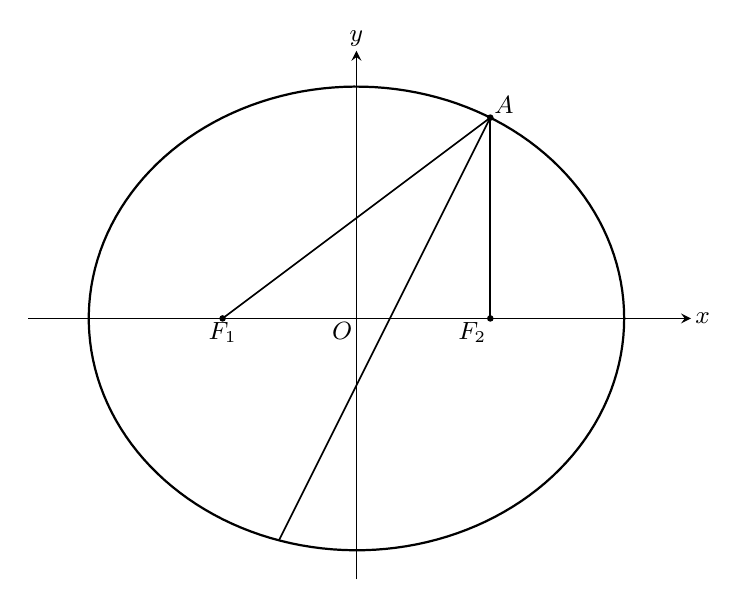
\begin{tikzpicture}[semithick, scale=0.85, every node/.style={inner sep=1.2pt, font=\small}]
  \draw[-stealth] (-4.9,0) -- (5.0,0) node[right] {$x$};
  \draw[-stealth] (0,-3.9) -- (0,4.0) node[above] {$y$};
  \draw[thick,domain=0:360,samples=160] plot ({4*cos(\x)},{3.4641*sin(\x)});
  \coordinate (A) at (2,3);
  \coordinate (F1) at (-2,0);
  \coordinate (F2) at (2,0);
  \coordinate (P) at (-1.1579,-3.3158);
  \draw (A) -- (F1);
  \draw (A) -- (F2);
  \draw (A) -- (P);
  \fill (A) circle (1.4pt);
  \fill (F1) circle (1.4pt);
  \fill (F2) circle (1.4pt);
  \node[above right] at (A) {$A$};
  \node[below] at (F1) {$F_1$};
  \node[below left] at (F2) {$F_2$};
  \node[below left] at (0,0) {$O$};
\end{tikzpicture}
\end{center}
\nopagebreak[4]
\Needspace{4\baselineskip}
\textbf{解析}

先由离心率把 $b^2$ 用 $a^2$ 表示，再用过点条件定 $a^2$。

\Needspace{5\baselineskip}
（1）设椭圆为 $\dfrac{x^2}{a^2}+\dfrac{y^2}{b^2}=1$（$a>b>0$）。由 $e=\dfrac ca=\dfrac12$ 得 $c=\dfrac a2$，故

\nopagebreak[4]
\[b^2=a^2-c^2=\frac34a^2.\]

\Needspace{5\baselineskip}
代入 $A(2,3)$：

\nopagebreak[4]
\[\frac4{a^2}+\frac9{\frac34a^2}=1
\Longrightarrow \frac{16}{a^2}=1
\Longrightarrow a^2=16.\]

\Needspace{5\baselineskip}
于是 $b^2=12$，椭圆为

\nopagebreak[4]
\[\frac{x^2}{16}+\frac{y^2}{12}=1.\]

\Needspace{5\baselineskip}
（2）由（1）$c=2$，故 $F_1(-2,0)$，$F_2(2,0)$，且

\nopagebreak[4]
\[\overrightarrow{AF_1}=(-4,-3),\qquad \overrightarrow{AF_2}=(0,-3).\]

\Needspace{5\baselineskip}
两方向的单位向量分别为 $\left(-\dfrac45,-\dfrac35\right)$ 与 $(0,-1)$，其和为 $\left(-\dfrac45,-\dfrac85\right)$，方向为 $(-1,-2)$。故角平分线的斜率为 $2$，方程为

\nopagebreak[4]
\[y-3=2(x-2),\]

即 $2x-y-1=0$。

\gkanswer{答案：（1）$\dfrac{x^2}{16}+\dfrac{y^2}{12}=1$；（2）$2x-y-1=0$。}

\end{answer}
\begin{answer}
\gksolhead{18}{}

\textbf{题目}：

某市 $2010$ 年 $4$ 月 $1$ 日 — $4$ 月 $30$ 日对空气污染指数的监测数据如下（主要污染物为可吸入颗粒物）：

$61$，$76$，$70$，$56$，$81$，$91$，$92$，$91$，$75$，$81$，$88$，$67$，$101$，$103$，$95$，$91$，$77$，$86$，$81$，$83$，$82$，$82$，$64$，$79$，$86$，$85$，$75$，$71$，$49$，$45$。

（1）完成频率分布表；

（2）作出频率分布直方图；

（3）根据国家标准，污染指数在 $0\sim50$ 之间时，空气质量为优；在 $51\sim100$ 之间时，为良；在 $101\sim150$ 之间时，为轻微污染；在 $151\sim200$ 之间时，为轻度污染。请你依据所给数据和上述标准，对该市的空气质量给出一个简短评价。

\Needspace{4\baselineskip}
\textbf{解析}

先按组距 $10$ 分组统计频数，再算频率与频率/组距。

（1）数据最小值为 $45$，最大值为 $103$，取分组 $[40,50)$，$[50,60)$，$\cdots$，$[100,110)$。各组频数为 $2,1,3,7,10,5,2$，频率依次为 $\dfrac1{15},\dfrac1{30},\dfrac1{10},\dfrac7{30},\dfrac13,\dfrac16,\dfrac1{15}$。列成频率分布表：

\begin{center}
\begin{tabular}{llll}
\toprule
分组 & 频数 & 频率 & 频率/组距 \\
\midrule
$[40,50)$ & $2$ & $\frac1{15}$ & $\frac1{150}$ \\
$[50,60)$ & $1$ & $\frac1{30}$ & $\frac1{300}$ \\
$[60,70)$ & $3$ & $\frac1{10}$ & $\frac1{100}$ \\
$[70,80)$ & $7$ & $\frac7{30}$ & $\frac7{300}$ \\
$[80,90)$ & $10$ & $\frac13$ & $\frac1{30}$ \\
$[90,100)$ & $5$ & $\frac16$ & $\frac1{60}$ \\
$[100,110)$ & $2$ & $\frac1{15}$ & $\frac1{150}$ \\
\bottomrule
\end{tabular}
\end{center}

（2）以横轴表示污染指数、纵轴表示频率/组距，在每一组上作高等于该组频率/组距的矩形，即得频率分布直方图。

（3）污染指数在 $0\sim50$ 的有 $2$ 天，占 $\dfrac1{15}$；在 $51\sim100$ 的有 $26$ 天，占 $\dfrac{13}{15}$；在 $101\sim150$ 的有 $2$ 天，占 $\dfrac1{15}$；没有轻度污染的天数。优、良天数合计占 $\dfrac{14}{15}$，故该市空气质量总体为良。

\gkanswer{答案：（1）频率分布表如下；（2）直方图如下；（3）空气质量总体为良。}

\end{answer}
\begin{answer}
\gksolhead{19}{}

\textbf{题目}：

如图，在多面体 $ABCDEF$ 中，四边形 $ABCD$ 是正方形，$EF\parallel AB$，$EF\perp FB$，$AB=2EF$，$\angle BFC=90^\circ$，$BF=FC$，$H$ 为 $BC$ 的中点。

（1）求证：$FH\parallel$ 平面 $EDB$；

（2）求证：$AC\perp$ 平面 $EDB$；

（3）求四面体 $B-DEF$ 的体积。
\nopagebreak[4]
\begin{center}% 2010 年安徽卷文科第 19 题：多面体 ABCDEF，H 为 BC 中点。
% 来源 PDF：普通高考/2010/2010安徽文.pdf，SHA-256 1bd928e09356787e648fa9efb9b4c1525f26334f65b08ba82fc736ebb110a4cb。
% 原页：第 2 页（A3 三栏）第 1 栏下部，书页码 572。
% 重绘依据：ABCD 为正方形，EF∥AB，EF⊥FB，AB=2EF，∠BFC=90°，BF=FC；
%   取 AB=2、EF=1，F(2,1,1)、E(1,1,1)，投影 x_s=x+0.45y、y_s=0.55z+0.45y；
%   可见棱实线，被遮挡的 DC 与辅助线 AC、BD、DF 虚线，EB 与 FH 为实线。
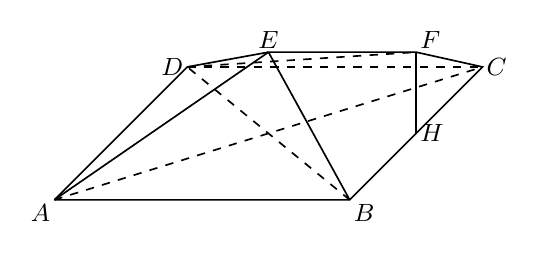
\begin{tikzpicture}[semithick, scale=1.25,
  every node/.style={inner sep=1.2pt, font=\small}]
  \coordinate (A) at (0,0);
  \coordinate (B) at (3,0);
  \coordinate (C) at (4.35,1.35);
  \coordinate (D) at (1.35,1.35);
  \coordinate (E) at (2.175,1.50);
  \coordinate (F) at (3.675,1.50);
  \coordinate (H) at (3.675,0.675);
  % 可见棱
  \draw (A) -- (B) -- (C) -- (F) -- (E) -- (A);
  \draw (A) -- (D) -- (E);
  \draw (B) -- (E);
  \draw (F) -- (H);
  % 被遮挡的棱与辅助线
  \draw[dashed] (D) -- (C);
  \draw[dashed] (A) -- (C);
  \draw[dashed] (B) -- (D);
  \draw[dashed] (D) -- (F);
  % 顶点标注
  \node[below left] at (A) {$A$};
  \node[below right] at (B) {$B$};
  \node[right] at (C) {$C$};
  \node[left] at (D) {$D$};
  \node[above] at (E) {$E$};
  \node[above right] at (F) {$F$};
  \node[right] at (H) {$H$};
\end{tikzpicture}
\end{center}
\nopagebreak[4]
\Needspace{4\baselineskip}
\textbf{解析}

取 $AB=2$，建立空间直角坐标系，把平行与垂直都化为向量计算。

\Needspace{5\baselineskip}
设正方形边长 $AB=2$，则 $EF=1$。以 $A$ 为原点，$AB$，$AD$ 为 $x$，$y$ 轴正方向，过 $A$ 垂直于底面的方向为 $z$ 轴正方向，则

\nopagebreak[4]
\[A(0,0,0),\quad B(2,0,0),\quad C(2,2,0),\quad D(0,2,0).\]

\Needspace{5\baselineskip}
由 $BF=FC$，$\angle BFC=90^\circ$，$BC=2$ 得 $BF=FC=\sqrt2$，故 $F$ 在 $BC$ 的垂直平分面上且到底面距离为 $1$，取

\nopagebreak[4]
\[F(2,1,1).\]

\Needspace{5\baselineskip}
又 $EF\parallel AB$ 且 $EF=1$，取 $E(1,1,1)$。此时

\nopagebreak[4]
\[\overrightarrow{EF}=(1,0,0),\qquad \overrightarrow{FB}=(0,-1,-1),\]

故 $\overrightarrow{EF}\cdot\overrightarrow{FB}=0$，即 $EF\perp FB$，与题设相符。

（1）$H$ 为 $BC$ 中点，故 $H(2,1,0)$，$\overrightarrow{FH}=(0,0,-1)$。

\Needspace{5\baselineskip}
在平面 $EDB$ 中，

\nopagebreak[4]
\[\overrightarrow{ED}=(-1,1,-1),\qquad \overrightarrow{EB}=(1,-1,-1),\]

\Needspace{5\baselineskip}
取法向量

\nopagebreak[4]
\[\boldsymbol n=\overrightarrow{ED}\times\overrightarrow{EB}=(-2,-2,0),\]

\Needspace{5\baselineskip}
可简化为 $(1,1,0)$。因

\nopagebreak[4]
\[\overrightarrow{FH}\cdot\boldsymbol n=0,\]

故 $FH$ 与平面 $EDB$ 平行或在其内。又 $F(2,1,1)$ 满足 $x+y=3\neq2$，不在平面 $EDB$（$x+y=2$）内，所以 $FH\parallel$ 平面 $EDB$。

（2）$\overrightarrow{AC}=(2,2,0)=2(1,1,0)$，与平面 $EDB$ 的法向量平行；且 $A(0,0,0)$ 不在平面 $EDB$ 内，故 $AC\perp$ 平面 $EDB$。

\Needspace{5\baselineskip}
（3）由

\nopagebreak[4]
\[\overrightarrow{BD}=(-2,2,0),\quad \overrightarrow{BE}=(-1,1,1),\quad \overrightarrow{BF}=(0,1,1),\]

\Needspace{5\baselineskip}
得

\nopagebreak[4]
\[\overrightarrow{BE}\times\overrightarrow{BF}=(0,1,-1),\]

\Needspace{5\baselineskip}
故

\nopagebreak[4]
\[\overrightarrow{BD}\cdot(\overrightarrow{BE}\times\overrightarrow{BF})=2.\]

\Needspace{5\baselineskip}
于是四面体 $B-DEF$ 的体积

\nopagebreak[4]
\[V=\frac16\left|\overrightarrow{BD}\cdot(\overrightarrow{BE}\times\overrightarrow{BF})\right|=\frac16\times2=\frac13.\]

\gkanswer{答案：（1）证明；（2）证明；（3）$\dfrac13$。}

\end{answer}
\begin{answer}
\gksolhead{20}{}

\textbf{题目}：

设函数 $f(x)=\sin x-\cos x+x+1$，$0<x<2\pi$，求函数 $f(x)$ 的单调区间与极值。

\Needspace{4\baselineskip}
\textbf{解析}

\Needspace{5\baselineskip}
先求导并化为一个正弦型函数，再解 $f'(x)>0$ 与 $f'(x)<0$。

\nopagebreak[4]
\[f'(x)=\cos x+\sin x+1=\sqrt2\sin\left(x+\frac\pi4\right)+1.\]

\Needspace{5\baselineskip}
当 $0<x<2\pi$ 时，$x+\dfrac\pi4\in\left(\dfrac\pi4,\dfrac{9\pi}4\right)$。由

\nopagebreak[4]
\[\sin\left(x+\frac\pi4\right)>-\frac{\sqrt2}2\]

\Needspace{5\baselineskip}
得

\nopagebreak[4]
\[x\in(0,\pi)\cup\left(\frac{3\pi}2,2\pi\right);\]

在该范围内 $f'(x)>0$。当 $x\in\left(\pi,\dfrac{3\pi}2\right)$ 时 $f'(x)<0$。故 $f$ 在 $(0,\pi)$ 与 $\left(\dfrac{3\pi}2,2\pi\right)$ 上单调递增，在 $\left(\pi,\dfrac{3\pi}2\right)$ 上单调递减。

\Needspace{5\baselineskip}
极大值为

\nopagebreak[4]
\[f(\pi)=0-(-1)+\pi+1=\pi+2,\]

\Needspace{5\baselineskip}
极小值为

\nopagebreak[4]
\[f\left(\frac{3\pi}2\right)=-1-0+\frac{3\pi}2+1=\frac{3\pi}2.\]

\gkanswer{答案：增区间为 $(0,\pi)$ 与 $\left(\dfrac{3\pi}2,2\pi\right)$，减区间为 $\left(\pi,\dfrac{3\pi}2\right)$；极大值 $\pi+2$，极小值 $\dfrac{3\pi}2$。}

\end{answer}
\begin{answer}
\gksolhead{21}{}

\textbf{题目}：

设 $C_1$，$C_2$，$\cdots$，$C_n$，$\cdots$ 是坐标平面上的一列圆，它们的圆心都在 $x$ 轴的正半轴上，且都与直线 $y=\dfrac{\sqrt3}3x$ 相切，对每一个正整数 $n$，圆 $C_n$ 都与圆 $C_{n+1}$ 相互外切，以 $r_n$ 表示 $C_n$ 的半径，已知 $\{r_n\}$ 为递增数列。

（1）证明：$\{r_n\}$ 为等比数列；

（2）设 $r_1=1$，求数列 $\left\{\dfrac{n}{r_n}\right\}$ 的前 $n$ 项和。
\nopagebreak[4]
\begin{center}% 2010 年安徽卷文科第 21 题：圆心在 x 轴正半轴上、与直线 y=(√3/3)x 相切的一列外切圆。
% 来源 PDF：普通高考/2010/2010安徽文.pdf，SHA-256 1bd928e09356787e648fa9efb9b4c1525f26334f65b08ba82fc736ebb110a4cb。
% 原页：第 2 页（A3 三栏）第 3 栏中部，书页码 572。
% 重绘依据：r_{n+1}=3r_n，圆心横坐标 x_n=2r_n；图中按 r1=1 的比例画出前三个圆
%   （半径 1、3、9，按 0.18 缩放），三圆依次外切且均与直线相切。
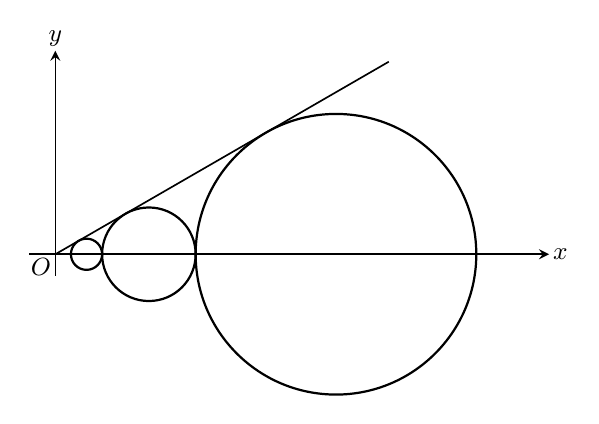
\begin{tikzpicture}[semithick, scale=1.1, every node/.style={inner sep=1.2pt, font=\small}]
  \draw[-stealth] (-0.3,0) -- (5.7,0) node[right] {$x$};
  \draw[-stealth] (0,-0.25) -- (0,2.35) node[above] {$y$};
  \draw (0,0) -- (3.85,2.223);
  \draw[thick] (0.36,0) circle (0.18);
  \draw[thick] (1.08,0) circle (0.54);
  \draw[thick] (3.24,0) circle (1.62);
  \node[below left] at (0,0) {$O$};
\end{tikzpicture}
\end{center}
\nopagebreak[4]
\Needspace{4\baselineskip}
\textbf{解析}

用圆心到切线的距离等于半径，把圆心横坐标用半径表示，再由外切条件建立递推。

\Needspace{5\baselineskip}
（1）设圆 $C_n$ 的圆心为 $(x_n,0)$，半径为 $r_n$。直线 $y=\dfrac{\sqrt3}3x$ 即 $x-\sqrt3y=0$，圆心到它的距离为

\nopagebreak[4]
\[\frac{x_n}{\sqrt{1+3}}=\frac{x_n}2.\]

\Needspace{5\baselineskip}
因圆与直线相切，

\nopagebreak[4]
\[r_n=\frac{x_n}2,\qquad x_n=2r_n.\]

\Needspace{5\baselineskip}
又圆 $C_n$ 与 $C_{n+1}$ 外切，故

\nopagebreak[4]
\[x_{n+1}-x_n=r_n+r_{n+1}.\]

\Needspace{5\baselineskip}
代入 $x_n=2r_n$：

\nopagebreak[4]
\[2r_{n+1}-2r_n=r_n+r_{n+1},\]

即 $r_{n+1}=3r_n$。因 $r_n>0$，故 $\{r_n\}$ 是公比为 $3$ 的等比数列。

\Needspace{5\baselineskip}
（2）由 $r_1=1$ 得 $r_n=3^{n-1}$，故

\nopagebreak[4]
\[S_n=\sum_{k=1}^n\frac{k}{r_k}=\sum_{k=1}^n\frac{k}{3^{k-1}}.\]

\Needspace{5\baselineskip}
两边乘 $\dfrac13$：

\nopagebreak[4]
\[\frac13S_n=\sum_{k=1}^n\frac{k}{3^k}.\]

\Needspace{5\baselineskip}
两式相减：

\nopagebreak[4]
\[\frac23S_n=\sum_{k=1}^n\frac1{3^{k-1}}-\frac{n}{3^n}
=\frac{1-\frac1{3^n}}{1-\frac13}-\frac{n}{3^n}
=\frac32\left(1-\frac1{3^n}\right)-\frac{n}{3^n}.\]

\Needspace{5\baselineskip}
故

\nopagebreak[4]
\[S_n=\frac94\left(1-\frac1{3^n}\right)-\frac{3n}{2\cdot3^n}
=\frac94-\frac{2n+3}{4\cdot3^{n-1}}.\]

\gkanswer{答案：（1）证明；（2）$\dfrac94-\dfrac{2n+3}{4\cdot3^{n-1}}$。}

\end{answer}